%%%%%%%% ICML 2024 EXAMPLE LATEX SUBMISSION FILE %%%%%%%%%%%%%%%%%

\documentclass{article}

% Recommended, but optional, packages for figures and better typesetting:
\usepackage{microtype}
\usepackage{tikz}
\usepackage{pgfplots}
\usepackage{graphicx}
\usepackage{subcaption}
\usepackage{booktabs} % for professional tables

% hyperref makes hyperlinks in the resulting PDF.
% If your build breaks (sometimes temporarily if a hyperlink spans a page)
% please comment out the following usepackage line and replace
% \usepackage{icml2024} with \usepackage[nohyperref]{icml2024} above.
\usepackage{hyperref}
\usepackage{multirow}

% Attempt to make hyperref and algorithmic work together better:
\newcommand{\theHalgorithm}{\arabic{algorithm}}

% Use the following line for the initial blind version submitted for review:
\usepackage{icml2024}

% If accepted, instead use the following line for the camera-ready submission:
% \usepackage[accepted]{icml2024}

% For theorems and such
\usepackage{amsmath}
\usepackage{amssymb}
\usepackage{mathtools}
\usepackage{amsthm}
\usepackage{bm}


% if you use cleveref..
\usepackage[capitalize,noabbrev]{cleveref}

%%%%%%%%%%%%%%%%%%%%%%%%%%%%%%%%
% THEOREMS
%%%%%%%%%%%%%%%%%%%%%%%%%%%%%%%%
\theoremstyle{plain}
\newtheorem{theorem}{Theorem}[section]
\newtheorem{proposition}[theorem]{Proposition}
\newtheorem{lemma}[theorem]{Lemma}
\newtheorem{corollary}[theorem]{Corollary}
\theoremstyle{definition}
\newtheorem{definition}[theorem]{Definition}
\newtheorem{assumption}[theorem]{Assumption}
\theoremstyle{remark}
\newtheorem{remark}[theorem]{Remark}

% Todonotes is useful during development; simply uncomment the next line
%    and comment out the line below the next line to turn off comments
%\usepackage[disable,textsize=tiny]{todonotes}
% \usepackage[textsize=tiny]{todonotes}


% The \icmltitle you define below is probably too long as a header.
% Therefore, a short form for the running title is supplied here:
\icmltitlerunning{Submission and Formatting Instructions for ICML 2024}

\DeclareMathOperator{\ilr}{ilr}
\DeclareMathOperator{\tr}{tr}

\begin{document}

\twocolumn[
\icmltitle{Explaining probabilistic predictions on the simplex with Shapley compositions}

% It is OKAY to include author information, even for blind
% submissions: the style file will automatically remove it for you
% unless you've provided the [accepted] option to the icml2024
% package.

% List of affiliations: The first argument should be a (short)
% identifier you will use later to specify author affiliations
% Academic affiliations should list Department, University, City, Region, Country
% Industry affiliations should list Company, City, Region, Country

% You can specify symbols, otherwise they are numbered in order.
% Ideally, you should not use this facility. Affiliations will be numbered
% in order of appearance and this is the preferred way.
\icmlsetsymbol{equal}{*}

\begin{icmlauthorlist}
\icmlauthor{Firstname1 Lastname1}{equal,yyy}
\icmlauthor{Firstname2 Lastname2}{equal,yyy,comp}
\icmlauthor{Firstname3 Lastname3}{comp}
\icmlauthor{Firstname4 Lastname4}{sch}
\icmlauthor{Firstname5 Lastname5}{yyy}
\icmlauthor{Firstname6 Lastname6}{sch,yyy,comp}
\icmlauthor{Firstname7 Lastname7}{comp}
%\icmlauthor{}{sch}
\icmlauthor{Firstname8 Lastname8}{sch}
\icmlauthor{Firstname8 Lastname8}{yyy,comp}
%\icmlauthor{}{sch}
%\icmlauthor{}{sch}
\end{icmlauthorlist}

\icmlaffiliation{yyy}{Department of XXX, University of YYY, Location, Country}
\icmlaffiliation{comp}{Company Name, Location, Country}
\icmlaffiliation{sch}{School of ZZZ, Institute of WWW, Location, Country}

\icmlcorrespondingauthor{Firstname1 Lastname1}{first1.last1@xxx.edu}
\icmlcorrespondingauthor{Firstname2 Lastname2}{first2.last2@www.uk}

% You may provide any keywords that you
% find helpful for describing your paper; these are used to populate
% the "keywords" metadata in the PDF but will not be shown in the document
\icmlkeywords{Machine Learning, ICML}

\vskip 0.3in
]

% this must go after the closing bracket ] following \twocolumn[ ...

% This command actually creates the footnote in the first column
% listing the affiliations and the copyright notice.
% The command takes one argument, which is text to display at the start of the footnote.
% The \icmlEqualContribution command is standard text for equal contribution.
% Remove it (just {}) if you do not need this facility.

%\printAffiliationsAndNotice{}  % leave blank if no need to mention equal contribution
\printAffiliationsAndNotice{\icmlEqualContribution} % otherwise use the standard text.

\begin{abstract}
  Shapley values have been widely used for explaining a machine learning model's prediction by measuring the contribution of each feature to the prediction. Coming from game theory, the Shapley value has been designed for a one-dimensional function's codomain. However, for a multiclass probabilistic classifier, the output is a discrete probability distribution, over a set of more than two possible classes, and lives on a multidimensional simplex. In this case, the Shapley values are sometimes computed on each output dimension one-by-one, in an implicit one-vs-rest setting, ignoring the compositional nature of the output distribution. Indeed, elements of the simplex are known as compositional data and a discrete probability distribution can therefore be treated as such taking into account the relative information between probabilities. Using the Aitchison geometry of the simplex, this paper presents an initiative for a multidimensional extension on the simplex of the concept of Shapley value, named Shapley composition, for explaining probabilistic predictions in machine learning.
\end{abstract}

\section{Introduction}

Many machine learning approaches---like the one based on deep learning or random forests---are often regarded as black-boxes making them unreliable for real-life applications where the model's predictions have to be understood or explainable. These recent years, the interest in more explainable models and explainability methods has therefore increased in the machine learning literature \cite{angelov2021explainable}. One group of approaches, known as \emph{local explanation}, aims to measure the contribution of each input feature to the computation of the model's output. Shapley values are widely used for this purpose \cite{vstrumbelj2014explaining,datta2016}, especially since the release of the SHAP toolkit \cite{NIPS2017_7062}\footnote{\url{https://github.com/shap/shap}}. The Shapley values come from cooperative game theory where a group of players work together to maximize a payoff. A set of Shapley values uniquely distributes the payoff over all the players according to their individual contribution to the total. Shapley value is known for respecting a set of desired axiomatic properties \cite{shapley1953value}. For explaining a machine learning model's prediction, a player becomes a feature and the total payoff is the scalar output of the model.

The concept of Shapley value is designed for a one-dimensional function's codomain. In game theory, the function takes a coalition of players and gives a gain or payoff. In machine learning, the function takes a group of features from an instance and gives a one-dimensional output or prediction. For two-classes classification models, the output is one-dimensional and usually given by a sigmoid transformation. The Shapley value framework can therefore simply be applied to the logit transformation of the model output. The logit transformation maps the sigmoid codomain $]0,1[$ to the real line $\mathbb{R}$. However, for classification tasks with more than two possible classes, the output of the model is multidimensional. This can be a discrete probability distribution or the output of a softmax layer commonly used in neural-networks. For a $N$-classes problem, these outputs live on a $(N-1)$-dimensional simplex. In this case, the Shapley value framework cannot be directly applied. Some apply the framework on each output probability one-by-one ignoring the structure of the simplex and the relative information between the probabilities.

Compositional data analysis \cite{aitchison1982,pawlowskymodeling} aims at treating data---known as compositions---living on a simplex. Compositional data analysis tools have been applied for instance on geological, and chemical data but also to discrete probability distributions \cite{egozcue2011evidence,egozcue2018evidence,noe2023representing}. This paper presents the use of the Aitchison geometry of the simplex, coming from the field of compositional data analysis, for extending the concept of Shapley value to the probability simplex, i.e.~the space of discrete probability distributions. This can be used to properly explain multiclass probabilistic prediction.

The next section of the paper, Section \ref{sec:shapley}, recalls the standard definition of the Shapley values, as applied to one-dimensional predictions in machine learning. Section \ref{sec:compo} presents the necessary tools from compositional data analysis, in particular, the Aitchison geometry of the simplex. Section \ref{sec:shapcompo} is the main contribution of the paper which is mostly theoretical. It defines, using the Aitchison geometry, the concept of Shapley composition for extending the Shapley value framework to the multidimensional simplex. Section \ref{sec:explain} shows, with simple examples and visualizations, how Shapley compositions can be used for explaining multidimensional probabilistic predictions in machine learning. Section \ref{sec:conclud} provides additional remarks and concludes the work.

\section{The Shapley values in machine learning}
\label{sec:shapley}

This section recalls the theoretical formulation of the Shapley values for measuring the contribution of each feature on a machine learning prediction.

Let $f:\mathcal{X}\to\mathbb{R}$ be a learned model one wants to \emph{locally} explain where $f(\bm{x})$ is the prediction on the instance $\bm{x}\in\mathcal{X}\subset\mathbb{R}^d$. Let $\text{Pr}$ be the probability distribution over $\mathcal{X}$ of the data\footnote{Usually, this is unknown but expectations will be replaced by empirical averagings.}. Let $S\subseteq \mathcal{I}=\{1,2,\dots d\}$ be a subset of indices where $d$ is the number of features. $\bm{x}_S$ refers to an instance $\bm{x}$ restricted to the features indicated by the indices in $S$.

When an instance $\bm{x}$ is observed, the expected value of the prediction is simply $\mathbb{E}[f(\bm{x}) \mid \bm{x}] = f(\bm{x})$. However, when only $\bm{x}_S$ is given with $\mathcal{S} \neq \mathcal{I}$, there is uncertainty about the non-observed features and we therefore compute the expected prediction given $\bm{x}_S$: $\mathbb{E}_{\text{Pr}}[f(\bm{x}) \mid \bm{x}_S] = \int_{\bm{x} \in \mathcal{X}}f(\bm{x})\text{Pr}(\bm{x} \mid \bm{x}_S)d\bm{x}$. The contribution of the feature indexed by $i \notin S$ in the prediction $f(\bm{x})$ given the known features indexed by $S$ is given by:
\begin{equation}
  \label{eq:contrib}
  c_{f,\bm{x},\text{Pr}}(i,\bm{X}_S) = v_{f,\bm{x},\text{Pr}}(\bm{X}_{S\cup\{i\}}) - v_{f,\bm{x},\text{Pr}}(\bm{X}_S),
\end{equation}
where $v$ is known as the value function:
\begin{equation}
  \label{eq:valuefunction}
  \begin{aligned}
    v_{f,\bm{x},\text{Pr}}: 2^{\mathcal{I}} &\to \mathbb{R},\\
    S &\mapsto \mathbb{E}_\text{Pr}[f(\bm{x})\mid \bm{x}_S],
  \end{aligned}
\end{equation}
where $2^{\mathcal{I}}$ is the set of all subsets of $\mathcal{I}$. This measures the contribution of the $i$th features with a particular \emph{coalition} of features indexed by $S$. The whole contribution of the $i$th feature is computed by averaging this quantity over all possible coalitions as follows:
\begin{equation}
  \phi_{f,\bm{x},\text{Pr}}(i) = \frac{1}{d!} \sum_{\pi}c_{f,\bm{x},\text{Pr}}(i,\pi^{<i}_{\bm{X}}),
\end{equation}
where $\pi$ is a permutation of the set $\mathcal{I}$ of indexes and $\pi^{<i}_{\bm{X}}$ is the features of $\bm{X}$ coming before the $i$th feature in the ordering given by $\pi$. For better clarity, the subscript $_{f,\bm{x},\text{Pr}}$ will be dropped from the equations.

This quantity is known as the Shapley value for the $i$th feature. It comes from cooperative game theory and is known to be the only quantity respecting a set of desired axiomatic properties \cite{shapley1953value}. It is linear as a function of the model ($\alpha, \beta \in \mathbb{R}$): $\phi_{\alpha f +\beta g}(i) = \alpha \phi_f(i) + \beta \phi_g(i)$, and the ``centered'' learned model is additively separable with respect to the Shapley values:
\begin{equation}
  f(\bm{x})-\mathbb{E}_{\text{Pr}}[f(\bm{X})] = \sum_{i=1}^{d} \phi_f(i),
\end{equation}
which is known as the \emph{efficiency} property.

The Shapley value is designed for a one-dimensional codomain of the function $f$. For explaining machine learning models which output multidimensional discrete probability distributions, like in multiclass classification, some people have been explaining each output dimension one-by-one, applying a logit transformation to the probabilities, resulting in a one-vs-rest comparison. However, this approach ignores the relative information between each probability and ignores the compositional nature of the discrete probability distributions. Indeed, the probabilistic output of a classifier lives on a multidimensional simplex. The latter is the sample space of \emph{compositional data} briefly reviewed in the next section.

\section{Compositional data}
\label{sec:compo}

Compositional data carries relative information. Each element of a composition \emph{describes a part of some whole} \cite{pawlowskymodeling} like vectors of proportions, concentrations, and discrete probability distributions. A $N$-part composition is a vector of $N$ non-zero positive real numbers that sum to a constant $k$. Each element of the vector is a part of the \emph{whole} $k$. The sample space of compositional data is the simplex: $\mathcal{S}^N = \left\{ \bm{x} = [x_1, x_2,\dots x_{N}]^T \in \mathbb{R}^{*N}_{+} \big| \sum_{i=1}^{N} x_i = k \right\}$. In a composition, only the relative information between parts matters and John Aitchison introduced the use of log-ratios of parts to handle this \cite{aitchison1982}. He defined several operations on the simplex which leads to what is called the \emph{Aitchison geometry of the simplex}.

\subsection{The Aitchison geometry of the simplex}
John Aitchison defined an internal operation called \emph{perturbation}, an external one called \emph{powering} and an inner product \cite{aitchison2001}:
\begin{itemize}
\item \emph{perturbation}:
  \begin{equation*}
    \bm{x}\oplus \bm{y} = \mathcal{C}\left([x_1y_1,\dots x_{N}y_{N}]\right),
  \end{equation*}
  seen as an addition between two compositions $\bm{x},\bm{y}\in \mathcal{S}^N$,
\item \emph{powering}:
  \begin{equation*}
    \alpha \odot \bm{x} = \mathcal{C}\left([x_{1}^{\alpha},\dots x_{N}^{\alpha}]\right),
  \end{equation*}
  seen as a multiplication by a scalar $\alpha \in \mathbb{R}$,
\item inner product:
  \begin{equation*}
    \langle \bm{x},\bm{y} \rangle_a = \frac{1}{2N}\sum_{i=1}^{N} \sum_{j=1}^{N} \log \frac{x_i}{x_j}\log \frac{y_i}{y_j},
  \end{equation*}
\end{itemize}
where $\mathcal{C}(\cdot)$ is the closure operator. Since only the relative information matter, scaling factors are irrelevant and a composition $\bm{x}$ is equivalent to $\lambda \bm{x} = [\lambda x_1,\lambda x_2,\dots\lambda x_N]$ for all $\lambda>0$. This equivalence is materialized by the closure operator defined for $k>0$ as: $\mathcal{C}\left(\bm{x} \right) = \left[ \frac{k x_1}{\lVert \bm{x} \rVert_1}, \frac{k x_2}{\lVert \bm{x} \rVert_1} ,\dots \frac{k x_N}{\lVert \bm{x} \rVert_1} \right]^T$, where $\bm{x} \in \mathbb{R}_+^{*N}$ and $\displaystyle \lVert \bm{x} \rVert_1 = \sum_{i=1}^N \lvert x_i \rvert$.%Therefore, any vector of positive real numbers can be projected onto the simplex using the closure.

This gives to the simplex a $(N-1)$-dimensional Euclidean vector space structure called \emph{Aitchison geometry of the simplex}. In this paper, since we are interested in classifiers' outputs as discrete probability distributions, we restrict ourselves to the \emph{probability simplex} where $k=1$.

\subsection{The isometric log-ratio transformation}
\label{sec:ilr}

An $(N-1)$-dimensional orthonormal basis of the simplex, referred to as an \emph{Aitchison} orthonormal basis, can be built. The projection of a composition into this basis defines an isometric isomorphism between $\mathcal{S}^N$ and $\mathbb{R}^{N-1}$. This is known as an Isometric-Log-Ratio (ILR) transformation \cite{egozcue2003isometric} and allows to express a composition into a Cartesian coordinates system preserving the metric of the Aitchison geometry. Within this real space, the permutation, the powering and the Aitchison inner product defined above are respectively the standard addition between two vectors, the multiplication of a vector by a scalar, and the standard inner product.

Given a composition $\bm{p} = \left[ p_1,\dots p_N \right]^T \in \mathcal{S}^N$ we write its ILR transformation as $\tilde{\bm{p}} = \ilr \left( \bm{p} \right) = \left[ \tilde{p}_1,\dots \tilde{p}_{N-1} \right]^T \in \mathbb{R}^{N-1}$. The $i$th element $\tilde{p}_i$ of $\tilde{\bm{p}}$ is obtained as: $\tilde{p}_i = \langle \bm{p}, \bm{e}^{(i)} \rangle_a$ where the set $\{\bm{e}^{(i)} \in \mathcal{S}^N, i=1,\dots N-1\}$ forms an \emph{Aitchison} orthonormal basis of the simplex. The choice of the basis will be discussed in Section \ref{sec:balances}.

\section{Shapley composition on the simplex}
\label{sec:shapcompo}

In Section \ref{sec:shapley} we have briefly presented the standard definition of the Shapley values in the context of machine learning one-dimensional predictions explanation. In this Section, we will see how the Aitchison geometry can be used to extend the concept of Shapley value to the simplex for explaining multidimensional probabilistic predictions.

Let $\bm{f}:\mathcal{X}\to\mathcal{S}^N$ be a learned model, like a $N$-classes probabilistic classifier for instance, which outputs a probabilistic prediction on the $(N-1)$-dimensional probability simplex $S^N$. In order to properly consider the structure of the simplex and the relative information between the probabilities, the output of the model must be treated as compositional data using the operators and metrics defined by the Aitchison geometry of the simplex. We therefore rewrite the contribution and the value function of Equations \ref{eq:contrib} and \ref{eq:valuefunction} as follows:
\begin{equation}
  \bm{c}_{\bm{f},\bm{x},\text{Pr}}(i,\bm{X}_S) = \bm{v}_{\bm{f},\bm{x},\text{Pr}}(\bm{X}_{S\cup\{i\}}) \ominus \bm{v}_{\bm{f},\bm{x},\text{Pr}}(\bm{X}_S),
\end{equation}
where $\bm{a}\ominus\bm{b}$ is the perturbation $\bm{a} \oplus \left( (-1)\odot \bm{b}\right)$ which correspond to a substraction between compositions $\bm{a}$ and $\bm{b}$, and where:
\begin{equation}
  \label{eq:valuefunctionsimplex}
  \begin{aligned}
    \bm{v}_{\bm{f},\bm{x},\text{Pr}}: 2^{\mathcal{I}} &\to \mathcal{S}^N,\\
    S &\mapsto \mathbb{E}^{\mathcal{A}}_\text{Pr}[\bm{f}(\bm{x})\mid \bm{x}_S].
  \end{aligned}
\end{equation}
The $\mathcal{A}$ in superscript highlights the fact that the expectation is done with respect to the Aitchison measure, rather than the Lebesgue measure, which can simply be computed as: $\mathbb{E}^{\mathcal{A}}[\bm{Y}] = \ilr^{-1}\left( \mathbb{E} \left[ \ilr\left( \bm{Y} \right) \right] \right)$,
where $\mathbb{E}^{\mathcal{A}}$ refers to the expectation with respect to the Aitchison measure while $\mathbb{E}$ refers to the expectation with respect to the Lebesgue measure \cite{pawlowskymodeling}.

The Shapley quantity expressing the contribution of the $i$th feature on a prediction can simply be expressed on the simplex as the composition $\bm{\phi}(i)$ given by:
\begin{equation}
  \bm{\phi}_{\bm{f},\bm{x},\text{Pr}}(i) = \frac{1}{d!} \odot \underset{\pi}{\bigoplus}\bm{c}_{\bm{f},\bm{x},\text{Pr}}(i,\pi^{<i}_{\bm{X}}).
\end{equation}
We call this quantity \emph{Shapley composition}. It can be shown (in Appendix \ref{app:properties}) that the linearity and the efficiency properties naturally hold for the Shapley composition:
\begin{equation}
  \begin{aligned}
    \bm{\phi}_{\alpha \odot \bm{f}(\bm{x}) \oplus \beta \odot \bm{g}(\bm{x})}(i) &= \alpha \odot \bm{\phi}_{\bm{f}}(i) \oplus \beta\odot \bm{\phi}_{\bm{g}}(i),\\
    \underset{i=1}{\overset{d}\bigoplus} \bm{\phi}_{\bm{f}}(i) &= \bm{f}(\bm{x}) \ominus \mathbb{E}^{\mathcal{A}}_{\text{Pr}}[\bm{f}(\bm{X})].
  \end{aligned}
\end{equation}
This can be seen as a multidimensional extension of the Shapley value framework on the simplex. Here, the Shapley quantity is not a scalar anymore, this is a composition living on the probability simplex. In the next section, we will see in more detail how this can be used to explain the contribution of each feature to a multidimensional probabilistic prediction.

\section{Explaining a prediction with Shapley compositions}
\label{sec:explain}

Given a probabilistic prediction $\bm{f}(\bm{x}) \in \mathcal{S}^N$, the Shapley composition $\bm{\phi}_{\bm{f},\bm{x},\text{Pr}}(i)$ describes the contribution of the $i$th feature on the prediction. The efficiency property shows how the probability distribution moves from the base distribution, i.e.~the expected prediction regardless of the current input, to the prediction $\bm{f}(\bm{x})$. In the standard Shapley formulation recalled in Section \ref{sec:shapley}, the prediction is one-dimensional such that the Shapley quantity is a scalar. In applications where there are more than two possible classes, the prediction is multidimensional such that the Shapley quantity is too. Both live in the same space: the probability simplex. In this section, we discuss how the set of Shapley compositions can be analysed to better understand the contribution and influence of each feature on the prediction.

\subsection{Visualization}

The Shapley compositions can be visualized in the Euclidean space isometric to the simplex thanks to the ILR transformation presented in Section \ref{sec:ilr}. As we will see, this space has the advantage of being intuitive since it is a standard real $(N-1)$-dimensional vector space.

\subsubsection{Three classes}

In a three-classes case, the space of the predictions is $2$-dimensional. We illustrate this example with the well-known Iris classification dataset consisting of a set of flowers described by 4 features: sepal length and width, and petal length and width. The aim of the classification task is to predict to which of the three species (setosa, versicolor and virginica) a flower belongs. In the present example, a Support Vector Machine (SVM) with a radial basis function (rbf) kernel and with pairwise coupling \cite{wu2003probability} is used as a probabilistic classifier. Figure \ref{fig:3classes} shows the explanation of the classifier prediction with one versicolor instance as input. Figure \ref{fig:3classesshap} shows the Shapley compositions in the ILR space and Figure \ref{fig:3classesshapsum} shows how they move the base distribution to the prediction. Having the highest norm, the petal length is the feature contributing the most to the prediction and moves the base distribution to the versicolor maximum probability decision region (maximum probability decision region boundaries are the dashed gray lines). Class-compositions are represented by color dashed vectors. A class-composition is defined as an unit norm composition going straight to the direction of one class and against all the others (see Appendix \ref{app:classcompo} for a formal definition). The Shapley composition for the petal length is orthogonal to the virginica class-composition, this suggests that this feature does not contribute to the predicted probability for this class. The Shapley composition for the petal width goes straight to the opposite direction of the setosa class-composition suggesting that this feature contributes to rejecting this class. The other Shapley compositions have a low norm suggesting that these features do not contribute to the prediction.
\begin{figure}
  \begin{subfigure}{0.5\textwidth}
    \centering
    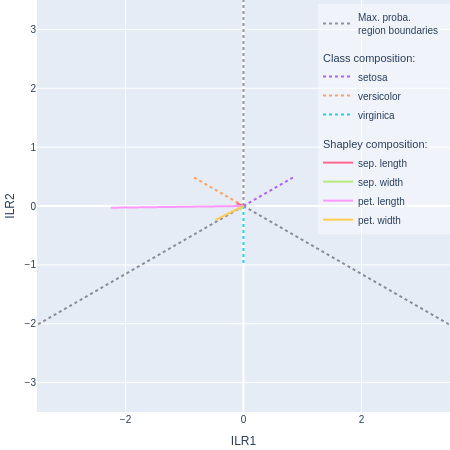
\includegraphics[width=0.8\linewidth]{figures/3classes/ilrplot.png}
    \caption{Shapley compositions in the ILR space.}
    \label{fig:3classesshap}
  \end{subfigure}
  
\vspace{0.5cm}
  \begin{subfigure}{0.5\textwidth}
    \centering
    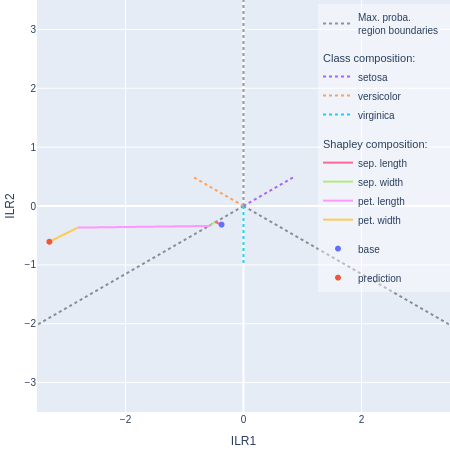
\includegraphics[width=0.8\linewidth]{figures/3classes/ilrplotsum.png}
    \caption{The sum of the Shapley compositions in the ILR space from the base distribution to the prediction.}
    \label{fig:3classesshapsum}
  \end{subfigure}
  \caption{Shapley explaination in the ILR space for the classification of an Iris instance.}
  \label{fig:3classes}
\end{figure}

\subsubsection{Four classes}

In a four-classes example, the simplex is $3$-dimensional. We illustrate this with a simple handwritten digit recognition task\footnote{We use the scikit-learn's digits dataset \cite{pedregosa2011scikit}.}. It consists of classifying an $8\times8$ image as representing one of the digits among 0, 1, 2 and 3. Since they are 64 pixels, considering each pixel as a feature would correspond to 64 Shapley compositions. This would be hard to visualize and analyse. We therefore reduce the number of features to 6 using a principal component analysis for better clarity and conciseness. A SVM with a rbf kernel and pairwise coupling is again used as a probabilistic classifier. The same explanation analysis as before can be applied here but within a $3$-dimensional plot as illustrated in Figure \ref{fig:4classesshapsum}. To better understand how this space is divided into four regions---each representing the maximum probability region for one class---one can think about the shape of a methane molecule. The hydrogens correspond to the vertices and the carbon to the center of a tetrahedron i.e.~a $3$-dimensional simplex. The relative positions of the class-compositions in the ILR space are the same as the bonds between the carbon and hydrogen: the angles are $\approx 109.5^{\circ}$. In this example, the tested instance is a 0\footnote{More examples can be obtained from the notebooks released on the git repository: link not shared during the double-blind peer reviewing.}.
\begin{figure}
  \centering
  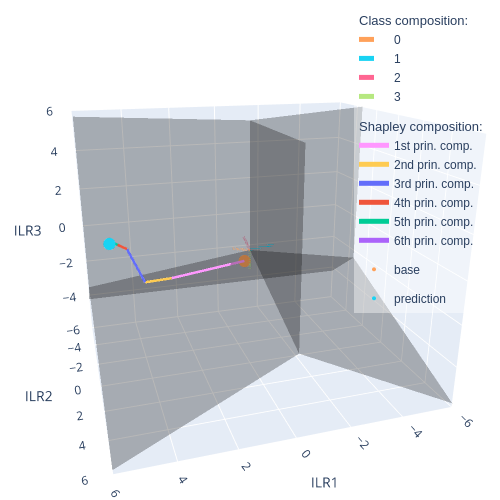
\includegraphics[width=0.9\linewidth]{figures/4classes/ilrplotsum.png}
  \caption{Shapley explaination in the $3$-dimensional ILR space for a four classes digit recognition task. The Shapley compositions are summed in the ILR space from the base distribution to the prediction. The gray transparent walls markout the maximum probability decision regions.}
  \label{fig:4classesshapsum}
\end{figure}

\subsection{More classes: groups of parts and balances}
\label{sec:balances}

When more than three classes are involved, all the dimensions of the ILR space cannot be visualized at once. However, $2$ or $3$-dimensional subspaces can still be visualized. In order to select the ILR components to investigate, one needs to understand what they refer to. In this section, we briefly discuss the interpretation of the ILR components.% of the explanation of a classifier prediction with more than three classes.

A component of the ILR space can be interpreted as a \emph{balance}, i.e.~a log-ratio of two geometrical means of parts \cite{egozcue2003isometric,egozcue2005groups,pawlowskymodeling}: one giving the central values of the probabilities in one group of classes and one for another group of classes. Therefore, a balance is here comparing the weight of two groups of classes. The set of balances is built such that they are geometrically orthogonal meaning they provide nonredundant information\footnote{Not to be confused with statistical uncorrelation \cite{pawlowskymodeling}.}.

This can be illustrated by a sequential binary partition or bifurcation tree. Figure \ref{fig:trees} gives two examples: \ref{fig:bifurc1} shows the bifurcation tree corresponding to the basis obtained with the Gram-Schmidt procedure as in \cite{egozcue2003isometric} which is the one used in the examples of Figures \ref{fig:3classes} and \ref{fig:4classesshapsum}  with respectively $N=3$ and $N=4$. Each node of the tree is a balance i.e.~an ILR component. The first balance $\tilde{p}_1$ first compares the probability for class $1$ with the probability for class $2$. Each next balance then recursively compares the probability for the next class with the probabilities for the previous classes independently of all the others.

In some applications, one may be interested in particular comparisons of groups of classes not necessarily given by a basis in the form of Figure \ref{fig:bifurc1}. For instance, as in an example presented in \cite{egozcue2005groups}, if one wants to compare political parties or groups, it may be pertinent to have a balance comparing left and right-wing groups. However, there are sometimes no obvious relevant comparisons to study. For instance, in the handwritten digit recognition problem, one may want to compare odd with even numbers or prime with non-prime but being basically a shape recognition problem, and the shape of the numbers being independent of their arithmetic properties, these comparisons are not pertinent. Be that as it may, the choice of the basis must be left open, whether or not it is based on a relevant strategy.

Let's use the basis of Figure \ref{fig:bifurc2} for a 10-classes digit recognition task\footnote{In this example, the bifurcation tree is obtained with agglomerative clustering of classes by recursively merging a pair of classes based on the Mahalanobis distance in the classifier's output space, assuming that within a pair of classes, the class-conditional densities are logistic-normal \cite{aitchison1980} with the same covariance matrix.}. We comment, for conciseness, a single $2$-dimensional subspace\footnote{More visualisations can be obtaned from the shared python notebooks.}. Let's have a look, in Figure \ref{fig:moreclasses35}, at the third and fifth ILR dimensions ($\tilde{p}_3$ and $\tilde{p}_5$). It is like saying we are only interested in comparing the probability assigned for class 0 with the probability assigned for class 6, and in comparing the probability assigned for class 1 with the group of probabilities assigned for classes 7 and 8. $\tilde{p}_3$ depends only on the probability for the digits 0 and 6 and $\tilde{p}_5$ depends only on the probabilities for the digits 1, 7 and 8. Therefore, the class-compositions for the other digits have a zero projection within this subspace and are therefore discarded in Figure \ref{fig:moreclasses35}. The class-compositions for 0 and 6 are orthogonal to the class-compositions for classes 1, 7 and 8. Indeed, the set of classes making the balance $\tilde{p}_3$ and the set of classes making $\tilde{p}_5$ have no intersection. In contrast, in the example of Figure \ref{fig:3classes}, $\tilde{p}_1$ is comparing the probabilities for the class setosa with the probability for the class versicolor and $\tilde{p}_2$ is comparing the probabilities for the class virginica with the group of probabilities for setosa and versicolor. In this case, none of the class-compositions are orthogonal. In Figure \ref{fig:moreclasses35}, since $\tilde{p}_5$ is comparing 1 with the group of digits 7 and 8, the projection on this line of the class-compositions for 1 goes in an opposite direction than the one for the class-compositions for 7 and 8. The latter two are equal and half as long as the former. In this way, $\tilde{p}_5$ compares the probability for 1 with the group of probabilities for 7 and 8 with the same weight. In other words, in this subspace, the class-compositions for 7 and 8 are reweighted such that this group of two classes has the same weight as the group made of the single class 1.

Within this space, Shapley compositions can be explored like in the examples of Figures \ref{fig:3classes} and \ref{fig:4classesshapsum} keeping in mind that this is a subset of the full ILR space. 
\begin{figure}
  \begin{subfigure}{0.5\textwidth}
    \centering
    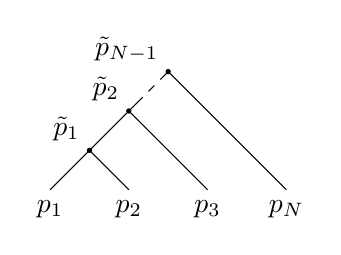
\begin{tikzpicture}[scale=1]
  \draw (0,0) -- (1.1,1.1);
  \draw[dashed] (1.1,1.1) -- (1.4,1.4);
  \draw (1.4,1.4) -- (1.5,1.5);
  \draw (0.5,0.5) -- (1,0);
  \draw (1,1) -- (2,0);
  \draw (1.5,1.5) -- (3,0);

  \filldraw[black] (0.5,0.5) circle (0.75pt) node[anchor=south east]{$\tilde{p}_{1}$};
  \filldraw[black] (1,1) circle (0.75pt) node[anchor=south east]{$\tilde{p}_{2}$};
  \filldraw[black] (1.5,1.5) circle (0.75pt) node[anchor=south east]{$\tilde{p}_{N-1}$};

  \draw[black] (0,-0.25) node{$p_1$};
  \draw[black] (1,-0.25) node{$p_2$};
  \draw[black] (2,-0.25) node{$p_3$};
  \draw[black] (3,-0.25) node{$p_{N}$};
\end{tikzpicture}


    \caption{Bifurcation tree corresponding to the basis obtained with the Gram-Schmidt procedure as in \cite{egozcue2003isometric} and used in the examples of Figures \ref{fig:3classes} and \ref{fig:4classesshapsum}.}
    \label{fig:bifurc1}
  \end{subfigure}

  \vspace{0.5cm}
  \begin{subfigure}{0.5\textwidth}
      \centering
      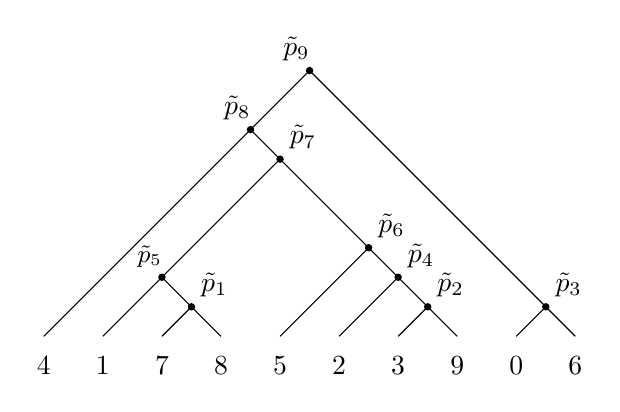
\begin{tikzpicture}[scale=1.5]
  \draw (0,0) -- (2.25,2.25);
  \draw (2.25,2.25) -- (4.5,0);
  \draw (2,1.5) -- (0.5,0);
  \draw (1.25,0.25) -- (1,0);
  \draw (1,0.5) -- (1.5,0);
  \draw (3.25,0.25) -- (3,0);
  \draw (4.25,0.25) -- (4,0);
  \draw (1.75,1.75) -- (3.5,0);
  \draw (3,0.5) -- (2.5,0);
  \draw (2.75,0.75) -- (2,0);
  
  \filldraw[black] (1.75,1.75) circle (0.75pt) node[label={[anchor=south east]0.1mm:$\tilde{p}_{8}$}]{};
  \filldraw[black] (2.25,2.25) circle (0.75pt) node[label={[anchor=south east]0.1mm:$\tilde{p}_{9}$}]{};
  \filldraw[black] (3.25,0.25) circle (0.75pt) node[anchor=south west]{$\tilde{p}_{2}$};
  \filldraw[black] (4.25,0.25) circle (0.75pt) node[anchor=south west]{$\tilde{p}_{3}$};
  \filldraw[black] (1.25,0.25) circle (0.75pt) node[anchor=south west]{$\tilde{p}_{1}$};
  \filldraw[black] (1,0.5) circle (0.75pt) node[label={[anchor=south east]0.1mm:\small $\tilde{p}_{5}$}]{};
  
  \filldraw[black] (2,1.5) circle (0.75pt) node[anchor=south west]{$\tilde{p}_{7}$};
  \filldraw[black] (3,0.5) circle (0.75pt) node[anchor=south west]{$\tilde{p}_{4}$};
  \filldraw[black] (2.75,0.75) circle (0.75pt) node[anchor=south west]{$\tilde{p}_{6}$};
  
  \draw[black] (0,-0.25) node{$4$};
  \draw[black] (0.5,-0.25) node{$1$};
  \draw[black] (1,-0.25) node{$7$};
  \draw[black] (1.5,-0.25) node{$8$};
  \draw[black] (2,-0.25) node{$5$};
  \draw[black] (2.5,-0.25) node{$2$};
  \draw[black] (3,-0.25) node{$3$};
  \draw[black] (3.5,-0.25) node{$9$};
  \draw[black] (4,-0.25) node{$0$};
  \draw[black] (4.5,-0.25) node{$6$};
\end{tikzpicture}


%%% Local Variables:
%%% mode: latex
%%% TeX-master: "main"
%%% End:

      \caption{Bifurcation tree used in the $10$-classes digit recognition task discussed in Section \ref{sec:balances} and in Figure \ref{fig:moreclasses35}.}
      \label{fig:bifurc2}
    \end{subfigure}
  \caption{Two examples of bifurcation tree.}
  \label{fig:trees}
\end{figure}
\begin{figure}
  \centering
  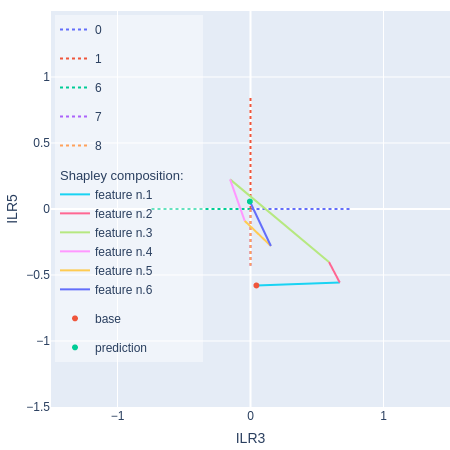
\includegraphics[width=0.8\linewidth]{figures/moreclasses/ilrplot35.png}
  \caption{The sum of the Shapley compositions from the base to the prediction in the ILR subspace made of $\tilde{p}_3$ and $\tilde{p}_5$ for a test instance from class 2. $\tilde{p}_3$ compares the probability assigned for class 0 with the probability assigned for class 6 and $\tilde{p}_5$ compares the probability assigned for class 1 with the group of probabilities assigned for class 7 and 8. The color dashed vectors represent the class-compositions with non-zero projection.}
  \label{fig:moreclasses35}
\end{figure}
\subsection{Angles, norms and projections}

Some may find the analysis of the features contributions in cases with more than four classes tricky. Indeed, in this case, the ILR space cannot be visualized in a $2$ or $3$-dimensional plot and as discussed in Section \ref{sec:balances}, choosing which subspaces to visualize require a careful understanding of the balances and a careful building of the bifurcation tree. However, the Shapley explaination can be summarized by sets of angles, norms and projections. The norm of a Shapley composition gives the strength of the feature's contribution in the prediction. It gives the overall contribution of the feature on the prediction, regardless of its direction. The angle between two Shapley compositions can informs about their orthogonality. If two Shapley composition are orthogonal%\footnote{We refer here to geometric orthogonality, not to be confused with statistical uncorrelation \cite{pawlowskymodeling}.}
, this suggest the features are nonredundant. A negative angle would suggest that the features have an opposite influence on the prediction. The projection of a Shapley composition on the set of class-compositions informs in favor of, or against, which classes a feature is contributing. Appendix \ref{app:summarize}, provides some examples of summarizing a Shapley explanation using the norm of Shapley compositions, angles between them and their projection on the class-compositions.

\subsection{Histograms}

If one found hard to visualize the proposed Shapley explanation in the ILR space, the Shapley composition can be visualized as histograms like discrete probability distributions. Figure \ref{fig:histiris} shows the Shapley compositions of the Iris classification example. The more uniform the histogram is, like for the sepal length and width, the less the contribution of the feature is. In opposite, the histogram for the petal length as a high value for the versicolor class, relatively to the others, confirming the contribution of the feature toward this class. For the petal width, the value for the class setosa is low relatively to the others which confirms the constribution of this feature against the class setosa.
\begin{figure}
  \centering
  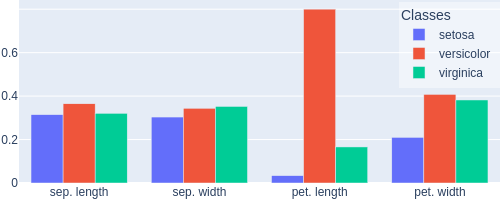
\includegraphics[width=0.9\linewidth]{figures/3classes/histo}
  \caption{Shapley compositions visualized as histograms for the Iris classification example.}
  \label{fig:histiris}
\end{figure}

As another illustration, Figure \ref{fig:histmore} shows the Shapley compositions of the $10$-classes digit recognition example. Contrary to the visualization of the compositions within the ILR space as discussed in Section \ref{sec:balances}, here, one can analyses all parts of each compositions within a single plot. In this example, the high of the class 2 for the first principal component confirms the contribution of this features toward this class.
\begin{figure}
  \centering
  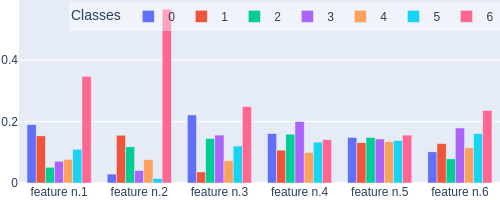
\includegraphics[width=0.9\linewidth]{figures/moreclasses/histo}
  \caption{Shapley compositions visualized as histograms for the seven classes digit recognition example.}
  \label{fig:histmore}
\end{figure}

\subsection{About our implementation}

In this work, the estimation algorithm we used to compute the Shapley compositions is an adaptation of Algorithm 2 in \cite{vstrumbelj2014explaining}. Since the resulting Shapley compositions are approximations, the efficiency property does not necessarily hold. Each Shapley composition is therefore corrected following a similar method as in the sampling approximation in the SHAP toolkit \cite{NIPS2017_7062}\footnote{\url{https://github.com/shap/shap/blob/master/shap/explainers/_sampling.py}} to respect the efficiency propery. See Appendix \ref{app:algo} and \ref{app:correct} for more details\footnote{The estimation algorithm we use assumes that the features are independent. We leave the exploration of estimation algorithms with no features-independence assumption for future work.}.

% \section{Shapley values versus Shapley composition}

\section{Discussion and conclusion}
\label{sec:conclud}

The use of standard Shapley value for explaining machine learning model with multidimensional probabilistic output has been rarely discussed in the literature. However, people computing a Shapley value on each output dimension one-by-one can be encounter. To be more precise, one may first found natural to compute a Shapley value on the logit of the probability for each classes resuilting in a $N$-dimensional vector of the Shapley values for a $N$-classes problem. Such vector will be refered here as \emph{Shapley vector}. Even if the efficiency property holds, i.e.~the sum of the element-wise logit of the base distribution with the Shapley vectors for each feature is equal to the element-wise logit of the prediction, the path from the base to the prediction may go out of the simplex which is conterintuitive. Indeed, this approach ignore the compositional nature of discrete probability distribution output by a classifier. Moreover, such strategy would require to run $N$ \emph{explanation model} contrary to our approach wich require a single explanation model.

As far as we know, this paper is the first work proposing an extension of the Shapley value framework to the multidimensional simplex for explaining probabilistic predictions in machine learning. We saw how the formalization of the standard Shapley value naturally extend to the simplex using the Aitchison geometry. The Shapley value therefore becomes a Shapley composition or distribution, i.e.~a vector living on the probability simplex. Such Shapley composition informs on the contribution of a feature on the prediction. It tells how the feature moves the distribution from the base one to the predicted one on the simplex. The Aitchison geometry defines on the simplex an Euclidean vector space structure such that the Shapley compositions can be analysed through angles, norms and projections.

The machine learning literature about the use of Shapley value is prolific. Many estimation algorithms have been developped, many applications of the Shapley value have emerged, and large scales experiments have been conducted. In contrast, our paper presents limited experimental results as simple proofs of concept and illustrations. However, we believe this work lies down proper theoretical foundations to foster researches in explainable machine learning especially for multiclass classification.

% In the unusual situation where you want a paper to appear in the
% references without citing it in the main text, use \nocite
\nocite{langley00}

\bibliography{biblio}
\bibliographystyle{icml2024}


%%%%%%%%%%%%%%%%%%%%%%%%%%%%%%%%%%%%%%%%%%%%%%%%%%%%%%%%%%%%%%%%%%%%%%%%%%%%%%%
%%%%%%%%%%%%%%%%%%%%%%%%%%%%%%%%%%%%%%%%%%%%%%%%%%%%%%%%%%%%%%%%%%%%%%%%%%%%%%%
% APPENDIX
%%%%%%%%%%%%%%%%%%%%%%%%%%%%%%%%%%%%%%%%%%%%%%%%%%%%%%%%%%%%%%%%%%%%%%%%%%%%%%%
%%%%%%%%%%%%%%%%%%%%%%%%%%%%%%%%%%%%%%%%%%%%%%%%%%%%%%%%%%%%%%%%%%%%%%%%%%%%%%%
\newpage
\appendix
\onecolumn

\section{Linearity and efficiency of the Shapley composition}
\label{app:properties}
In this section, we show the linearity of the Shapley composition with respect to the model prediction, and the efficiency property.

\subsection{Linearity}

The Shapley composition is linear, within the Aitchison geometry of the simplex, with respect to linear combination of models' predictions.
\begin{proof}
  Let's consider the linear combination of predictions $\bm{h}(\bm{x}) = \alpha \odot \bm{f}(\bm{x}) \oplus \beta \odot \bm{g}(\bm{x})$. we want to check if:
  \begin{equation}
    \label{eq:linearsimplex}
    \bm{\phi}_{\bm{h}}(i) = \alpha \odot \bm{\phi}_{\bm{f}}(i) \oplus \beta\odot \bm{\phi}_{\bm{g}}(i).
  \end{equation}
  We have:
  \begin{equation}
    \begin{aligned}
      \mathbb{E}^{\mathcal{A}}_{\text{Pr}}[\bm{h}(\bm{x})\mid \bm{x}_S] &= \ilr^{-1} \left( \mathbb{E}_{\text{Pr}} [\ilr \left(  \alpha \odot \bm{f}(\bm{x}) \oplus \beta \odot \bm{g}(\bm{x}) \right) \mid \bm{x}_S] \right),\\
                                                                        &= \ilr^{-1} \left( \mathbb{E}_{\text{Pr}} [\alpha \ilr \left( \bm{f}(\bm{x})\right) + \beta \ilr \left( \bm{g}(\bm{x}) \right) \mid \bm{x}_S] \right),\\
                                                                        &= \ilr^{-1} \left( \alpha \mathbb{E}_{\text{Pr}} [ \ilr \left( \bm{f}(\bm{x})\right) \mid \bm{x}_S] + \beta \mathbb{E}_{\text{Pr}} [ \ilr \left( \bm{g}(\bm{x}) \right) \mid \bm{x}_S] \right),\\
                                                                        &= \alpha \odot \ilr^{-1} \left( \mathbb{E}_{\text{Pr}} [ \ilr \left( \bm{f}(\bm{x})\right) \mid \bm{x}_S] \right) \oplus \beta \odot \ilr^{-1} \left( \mathbb{E}_{\text{Pr}} [ \ilr \left( \bm{g}(\bm{x}) \right) \mid \bm{x}_S] \right),\\
                                                                        &= \alpha \odot \mathbb{E}^{\mathcal{A}}_{\text{Pr}}[\bm{f}(\bm{x})\mid \bm{x}_S] \oplus \beta \odot \mathbb{E}^{\mathcal{A}}_{\text{Pr}}[\bm{g}(\bm{x})\mid \bm{x}_S].
    \end{aligned}
  \end{equation}
  Therefore, $\bm{v}_{\bm{h},\bm{x},\text{Pr}}(\bm{X}_S) = \alpha \odot \bm{v}_{\bm{f},\bm{x},\text{Pr}}(\bm{X}_S) \oplus \beta \odot \bm{v}_{\bm{g},\bm{x},\text{Pr}}(\bm{X}_S)$, meaning that $\bm{v}$ is linear with respect to the learned function or model. The linearity of the contribution $\bm{c}$ naturally follows:
  \begin{equation}
    \begin{aligned}
      &\bm{c}_{\bm{h},\bm{x},\text{Pr}}(i,\bm{X}_S) = \bm{v}_{\bm{h},\bm{x},\text{Pr}}(\bm{X}_{S\cup\{i\}}) \ominus \bm{v}_{\bm{h},\bm{x},\text{Pr}}(\bm{X}_S),\\
      &~~~~~~~= \left( \alpha \odot \bm{v}_{\bm{f},\bm{x},\text{Pr}}(\bm{X}_{S\cup\{i\}}) \oplus \beta \odot \bm{v}_{\bm{g},\bm{x},\text{Pr}}(\bm{X}_{S\cup\{i\}}) \right) \ominus \left( \alpha \odot \bm{v}_{\bm{f},\bm{x},\text{Pr}}(\bm{X}_S) \oplus \beta \odot \bm{v}_{\bm{g},\bm{x},\text{Pr}}(\bm{X}_S) \right),\\
      &~~~~~~~= \alpha \odot \bm{v}_{\bm{f},\bm{x},\text{Pr}}(\bm{X}_{S\cup\{i\}}) \oplus \beta \odot \bm{v}_{\bm{g},\bm{x},\text{Pr}}(\bm{X}_{S\cup\{i\}}) \ominus\alpha \odot \bm{v}_{\bm{f},\bm{x},\text{Pr}}(\bm{X}_S) \ominus \beta \odot \bm{v}_{\bm{g},\bm{x},\text{Pr}}(\bm{X}_S),\\
      &~~~~~~~= \alpha \odot \left( \bm{v}_{\bm{f},\bm{x},\text{Pr}}(\bm{X}_{S\cup\{i\}}) \ominus \bm{v}_{\bm{f},\bm{x},\text{Pr}}(\bm{X}_S) \right) \oplus \beta \odot \left( \bm{v}_{\bm{g},\bm{x},\text{Pr}}(\bm{X}_{S\cup\{i\}}) \ominus \bm{v}_{\bm{g},\bm{x},\text{Pr}}(\bm{X}_S)\right),\\
      &~~~~~~~= \alpha \odot \bm{c}_{\bm{f},\bm{x},\text{Pr}}(i,\bm{X}_S) \oplus \beta \odot \bm{c}_{\bm{g},\bm{x},\text{Pr}}(i,\bm{X}_S).
    \end{aligned}
  \end{equation}
  And the linearity of the Shap composition:
  \begin{equation}
    \begin{aligned}
      \bm{\phi}_{\bm{h}}(i) &= \frac{1}{d!}  \underset{\pi}{\bigoplus}\bm{c}_{\bm{h},\bm{x},\text{Pr}}(i,\pi^{<i}_{\bm{X}}),\\
                            &= \frac{1}{d!}  \underset{\pi}{\bigoplus}\left( \alpha \odot \bm{c}_{\bm{f},\bm{x},\text{Pr}}(i,\bm{X}_S) \oplus \beta \odot \bm{c}_{\bm{g},\bm{x},\text{Pr}}(i,\bm{X}_S) \right),\\
                            &= \alpha \odot \left( \frac{1}{d!}  \underset{\pi}{\bigoplus} \bm{c}_{\bm{f},\bm{x},\text{Pr}}(i,\bm{X}_S) \right) \oplus \beta \odot \left( \frac{1}{d!} \underset{\pi}{\bigoplus}    \bm{c}_{\bm{g},\bm{x},\text{Pr}}(i,\bm{X}_S) \right),\\
                            &= \alpha \odot \bm{\phi}_{\bm{f}}(i) \oplus \beta\odot \bm{\phi}_{\bm{g}}(i).
    \end{aligned}
  \end{equation}
\end{proof}

\newpage
\subsection{Efficiency}
The efficiency property naturally holds for Shapley compositions within the Aitchison geometry.
\begin{proof}
  \begin{equation}
    \begin{aligned}
      \underset{i=1}{\overset{d}\bigoplus} \bm{\phi}_{\bm{f}}(i) & = \underset{i=1}{\overset{d}\bigoplus}\left( \frac{1}{d!} \odot \underset{\pi}{\bigoplus} \bm{c}(i,\pi_{\bm{X}}^{<i})\right),\\
                                                                 &=  \frac{1}{d!} \odot \underset{i=1}{\overset{d}\bigoplus}\left( \underset{\pi}{\bigoplus} \left( \bm{v}(\pi_{\bm{X}}^{<i+1}) \ominus \bm{v}(\pi_{\bm{X}}^{<i}) \right) \right),\\
                                                                 &=  \frac{1}{d!} \odot \underset{i=1}{\overset{d}\bigoplus}\left( \underbrace{\left(\underset{\pi}{\bigoplus} \bm{v}(\pi_{\bm{X}}^{<i+1}) \right)}_{\bm{A}_{i+1}} \ominus \underbrace{\left( \underset{\pi}{\bigoplus} \bm{v}(\pi_{\bm{X}}^{<i}) \right)}_{\bm{A}_{i}} \right),\\
                                                                 &=  \frac{1}{d!} \odot \underset{i=1}{\overset{d}\bigoplus}\left( \bm{A}_{i+1} \ominus \bm{A}_{i} \right),\\
                                                                 &=  \frac{1}{d!} \odot \left( \bm{A}_{d+1} \ominus \bm{A}_{1} \right), \text{~since we have a telescoping perturbation,}\\
                                                                 &=  \frac{1}{d!} \odot \left( \left( \underset{\pi}{\bigoplus} \bm{v}(\pi_{\bm{X}}^{<d+1}) \right) \ominus \left( \underset{\pi}{\bigoplus} \bm{v}(\pi_{\bm{X}}^{<1}) \right) \right),\\
                                                                 &=  \frac{1}{d!} \odot \left( \left( \underset{\pi}{\bigoplus} \bm{v}(\bm{X}) \right) \ominus \left( \underset{\pi}{\bigoplus} \bm{v}(\bm{X}_{\emptyset}) \right) \right),\\
                                                                 &= \bm{v}(\bm{X}) \ominus \bm{v}(\bm{X}_{\emptyset}), \text{~since $d!$ is the number of different permutation,}\\
                                                                 &= \bm{f}(\bm{x}) \ominus \mathbb{E}^{\mathcal{A}}_{\text{Pr}}[\bm{f}(\bm{X})].
    \end{aligned}
  \end{equation}
\end{proof}


\newpage
\section{Class-compositions}
\label{app:classcompo}
A $k$-class-compositions $\bm{c}^{(k)}  \in \mathcal{S}^N$ is defined as an unit norm composition going straight to the direction of the $k$th class. This is a discrete probability distribution with maximum probability for the $k$th class and uniform values for the others. The $i$th part of the $\bm{c}^{(k)}$ is:
\begin{equation}
    c_i^{(k)} = \left\lbrace
  \begin{array}{@{}ll@{}}
    1-(N-1)p, & \text{if}\ i=k \\
    p, & \text{otherwise,}
  \end{array}\right.
\end{equation}
where $p<\frac{1}{N}$. We want the Aitchison norm of each class-composition to be one:
\begin{equation}
  \begin{aligned}
    \forall k \in \{1, \dots N \},~~~~~~\lVert \bm{c}^{(k)} \rVert_a = 1 \iff& \sqrt{\frac{1}{2N} \sum_{i=1}^N \sum_{j=1}^N \left( \log \frac{c_i^{(k)}}{c_j^{(k)}} \right)^2} = 1,\\
    \text{for clarity,}&\\\text{we drop the $(k)$ from the equations,}&\\
    \iff& \sqrt{\frac{1}{2N} \sum_{i=1}^{N}\left( \left(N-1 \right) \left( \log \frac{c_i}{p} \right)^2 + \left( \log \frac{c_i}{1-(N-1)p} \right)^2 \right)} = 1,\\
    \iff& \sqrt{\frac{1}{2N} 2(N-1) \left( \log \frac{p}{1-(N-1)p} \right)^2} =1,\\
    \text{since $p<\frac{1}{N}$ and the norm should be positive:}&\\
    \iff& \sqrt{\frac{N-1}{N}}\log \frac{1-(N-1)p}{p} =1,\\
    \iff& p = \frac{\exp \left( -\sqrt{\frac{N}{N-1}} \right)}{1+ (N-1)\exp \left( -\sqrt{\frac{N}{N-1}} \right )}.
  \end{aligned}
\end{equation}
To summarize, the $i$th part of a $k$-class-compositions $\bm{c}^{(k)} \in \mathcal{S}^N$ is given by:
\begin{equation}
    c_i^{(k)} =
  \frac{1}{1+ (N-1)\exp \left( -\sqrt{\frac{N}{N-1}} \right )} \left( \left\lbrace \begin{array}{@{}ll@{}}
     1, & \text{if}\ i=k \\
     \exp \left( -\sqrt{\frac{N}{N-1}} \right), & \text{otherwise,}
  \end{array}\right.\right).
\end{equation}
In this way, $\bm{c}^{(k)}$ is going straight to the direction of class $k$ and uniformly against all the others.


\newpage
\section{Summarizing the explanation with norms, angles and projections of Shapley compositions}
\label{app:summarize}

\begin{table}
  \centering
  \caption{Norm of the Shapley compositions, projection on the class-compositions and cosine similarity betweeen the Shapley compositions for the Iris classification example.}
  \begin{tabular}{c|c|ccc|cccc|}
    \cline{2-9}
    & \multirow{2}{*}{norm} & \multicolumn{3}{c|}{projection on the class-compositions} & \multicolumn{4}{c|}{cosine similarity between Shapley compositions} \\
    \cline{3-9}
     & & \small setosa & \small versicolor & \small virginica & \small pet. length & \small pet. width & \small sep. length & \small sep. width \\
    \hline
    \small pet. length & 2.20  & -1.91 & 1.90 & 0.02 & 1 &$\cdot$ &$\cdot$ &$\cdot$ \\
    \small pet. width & 0.51 & -0.51 & 0.29 & 0.22 & 0.90 & 1 &$\cdot$ &$\cdot$ \\
    \small sep. length & 0.13 & -0.08 & 0.13 & -0.05 & 0.93 & 0.69 & 1 &$\cdot$ \\
    \small sep. width & 0.11 & -0.11 & 0.04 & 0.07 & 0.77 & 0.97 & 0.49 &1 \\
    \hline
  \end{tabular}
  \label{tab:normiris}
\end{table}
The Table \ref{tab:normiris} gives, for the Iris classification example of Figure \ref{fig:3classes}, the norm of each Shapley compositions, the cosine similarity between them and their projection on the set of class-compositions. Having the highest norm, this confirms that the petal length is the feature that contributed the most on the prediction. Having a close to zero inner product with the virginica class-composition, shows that this feature did not contribute to the value of the probability of of this class. It contributes neither in favor, nor in the reject of this class. Having a positive inner product with the versicolor class-composition and a negative one with the setosa class-composition, this suggest that this feature is going in favor of the class versicolor and against setosa.

\begin{table}
  \centering
  \caption{Norm of the Shapley compositions and Cosine similarity betweeen the Shapley composition for the $10$-classes digit recognition example.}
  \begin{tabular}{c|c|cccccc|}
    \cline{2-8}
    & \multirow{2}{*}{norm} & \multicolumn{6}{c|}{cosine similarity between Shapley compositions} \\
    \cline{3-8}
     & & \small feature n.1 & \small feature n.2 & \small feature n.3 & \small feature n.4 & \small feature n.5 & \small feature n.6 \\
    \hline
    \small feature n.1 & 4.00 & 1 & $\cdot$ & $\cdot$ & $\cdot$ & $\cdot$ & $\cdot$ \\
    \small feature n.2 & 1.15 & -0.17 & 1 & $\cdot$ & $\cdot$ & $\cdot$ & $\cdot$ \\
    \small feature n.3 & 2.25 & 0.24 & 0.23 & 1 & $\cdot$ & $\cdot$ &$\cdot$ \\
    \small feature n.4 & 1.26 & -0.23 & 0.23 & 0.09 & 1 & $\cdot$ & $\cdot$ \\
    \small feature n.5 & 0.60 & 0.18  & -0.17 & -0.01 & -0.56 & 1 & $\cdot$ \\
    \small feature n.6 & 1.11 & 0.14 & 0.35 &	-0.19 & -0.03 & -0.48 & 1 \\
    \hline
  \end{tabular}
  \label{tab:normdigit}
\end{table}

\begin{table}
  \centering
  \caption{Projection of the Shapley compositions on the class-compositions for the $10$-classes digit recognition example.}
  \begin{tabular}{c|cccccccccc|}
    \cline{2-11}
    & \multicolumn{10}{c|}{projection on the class-compositions} \\
    \cline{2-11}
    & 0 & 1 & 2 & 3 & 4 & 5 & 6 & 7 & 8 & 9 \\
    \hline
    \small feature n.1 & 1.65 & -0.85 & 0.09 & -0.57 & -1.92 & -0.34 & 1.74 & 1.96 & 0.22 & -1.81 \\
    \small feature n.2 & -0.50 & 0.35 & 0.11 & 0.08 & -0.57 & -0.29 & -0.10 & 0.33 & -0.14 & 0.74\\
    \small feature n.3 & 0.36 & 0.45 & 0.23 & 1.20 & -1.37 & -0.56 & 0.91 & -0.83 & -0.31 & -0.09 \\
    \small feature n.4 & 0.19 & 0.02 & 0.61 & 0.18 & -0.53 & 0.46 & -0.86 & -0.17 & -0.12 & 0.22 \\
    \small feature n.5 & -0.03 & -0.02 & -0.22 & -0.31 & -0.02 & 0.13 & 0.42 & -0.16& 0.14 & 0.07 \\
    \small feature n.6 & -0.17 & 0.34 & -0.22 & 0.17 & -0.12 & -0.43 &-0.50  & 0.75 & 0.34 & -0.18 \\
    \hline
  \end{tabular}
  \label{tab:projdigit}
\end{table}
Table \ref{tab:normdigit} shows, for the $10$-classes digit recognition example, the norm of each Shapley composition and the cosine similarity between the, and Table \ref{tab:projdigit} shows their projection of the set of class-compositions.\\
Add details...

\newpage
\section{Estimation of the Shapley compositions}
\label{app:algo}
In this section, we present an adaptation of Algorithm 2 from \cite{vstrumbelj2014explaining} we used for the estimation the Shapley compositions.

Let $d$ be the number of features. We want to optimally distribute the $m_{\text{max}}$ drawn samples over the $d$ features. Let $\hat{\bm{\phi}_i}$ be the estimation of the Shapley composition for the $i$th feature. We want to minimize the sum of squared errors: $\displaystyle\sum_{i=1}^{d} \| \hat{\bm{\phi}_i} \ominus \bm{\phi}_i \|_a^2$. Since $\hat{\bm{\phi}_i}$ is a (Aitchison) sample mean we have: $\tilde{\hat{\bm{\phi}_i}} \approx \mathcal{N}(\tilde{\bm{\phi}}_i, \frac{1}{m_i}\bm{\Sigma}^{(i)})$ and $\tilde{\hat{\bm{\phi}_i}} - \tilde{\bm{\phi}}_i \approx \mathcal{N}(\bm{0}, \frac{1}{m_i}\bm{\Sigma}^{(i)})$ where the tilde refers to the ILR transformation.
Let $\bm{\Delta_i} = \tilde{\hat{\bm{\phi}_i}} - \tilde{\bm{\phi}}_i$ and $Z_i = \| \hat{\bm{\phi}_i} \ominus \bm{\phi}_i \|_a = \| \tilde{\hat{\bm{\phi}_i}} - \tilde{\bm{\phi}}_i \|_2 = \| \bm{\Delta}_i \|_2$. The expectation of the sum of squared errors is:
\begin{equation}
  \begin{aligned}
    \mathbb{E}\left[ \sum_{i=1}^{d} Z_i^2 \right] &=   \sum_{i=1}^{d} \mathbb{E}\left[ Z_i^2 \right],\\
                                                  & =\sum_{i=1}^{d} \mathbb{E}\left[ \sum_{j=1}^{d-1}\Delta_{ij}^2 \right],\\
                                                  & =\sum_{i=1}^{d} \sum_{j=1}^{d-1} \mathbb{E}\left[\Delta_{ij}^2 \right],\\
                                                  & =\sum_{i=1}^{d} \sum_{j=1}^{d-1} \frac{1}{m_i}\Sigma_{jj}^{(i)}, \text{ since } \Delta_{ij}\approx \mathcal{Z}(0, \frac{1}{m_i}\Sigma_{jj}^{(i)}),\\
    &= \sum_{i=1}^d \frac{1}{m_i} \tr \bm{\Sigma}^{(i)}.
  \end{aligned}
\end{equation}

When a sample is drawn, the feature for which the sample will be used for improving the Shapley composition estimation is chosen to maximize $\frac{\tr \bm{\Sigma}^{(i)}}{m_i} - \frac{\tr \bm{\Sigma}^{(i)}}{m_i+1}$. Like in \cite{vstrumbelj2014explaining}, this is summarized in Algorithm \ref{alg:2}.
\begin{algorithm}
   \caption{Adaptation of the Algorithm 1 from \cite{vstrumbelj2014explaining} for approximating the Shapley composition of the $i$th feature, with model $\bm{f}$, instance $\bm{x}\in\mathcal{X}$ and $m$ drawn samples.}
   \label{alg:1}
\begin{algorithmic}
   \STATE Initialize $\bm{\phi_i}\leftarrow \ilr^{-1}(\bm{0})$
   \FOR{$1$ {\bfseries to} $m$}
   \STATE Randomly select a permutation $\pi$ of the set of indexes $\mathcal{I}$,
   \STATE Randomly select a sample $\bm{w}\in\mathcal{X}$,
   \STATE Construct two instances:
   \begin{itemize}
     \item $\bm{b}_1$: which takes the values from $\bm{x}$ for the $i$th feature and the features indexed before $i$ in the order given by $\pi$, and takes the values from $\bm{w}$ otherwise,
     \item $\bm{b}_2$: which takes the values from $\bm{x}$ the features indexed before $i$ in the order given by $\pi$, and takes the values from $\bm{w}$ otherwise.
     \end{itemize}
   \STATE $\bm{\phi}_i \leftarrow \bm{\phi}_i \oplus \bm{f}(\bm{b}_1) \ominus \bm{f}(\bm{b}_2) $
   \ENDFOR
   \STATE $\bm{\phi}_i \leftarrow \frac{\bm{\phi}_i}{m}$
\end{algorithmic}
\end{algorithm}

\begin{algorithm}
   \caption{Adaptation of the Algorithm 2 from \cite{vstrumbelj2014explaining} for approximating all the Shapley compositions by optimally distributing a maximum number of samples $m_{\text{max}}$ over the $d$ features, with model $\bm{f}$, instance $\bm{x}\in\mathcal{X}$ and $m_{\text{min}}$ the minimum number of samples each feature estimation.}
   \label{alg:2}
   \begin{algorithmic}
     \STATE Initialization: $m_{i} \leftarrow 0$, $\bm{\phi}_i \leftarrow \bm{0}$, $\forall i \in \{1, \dots d\}$,
     \WHILE{$\displaystyle \sum_{i=1}^d m_i < m_{\text{max}}$}
     \IF{$\forall i, m_i \leq m_{\text{min}}$}
     \STATE $j = \underset{i}{\text{argmax}} \left( \frac{\tr \bm{\Sigma}^{(i)}}{m_i} - \frac{\tr \bm{\Sigma}^{(i)}}{m_i+1} \right)$,
     \ELSE
     \STATE pick a $j$ such that $m_j < m_{\text{min}}$,
     \ENDIF
     \STATE $\bm{\phi}_j \leftarrow \bm{\phi}_j$ $+$ result of Algorithm \ref{alg:1} for the $j$th feature and $m=1$,
     \STATE update $\bm{\Sigma}^{(j)}$ using an incremental algorithm,
     \STATE $m_j \leftarrow m_j+1$
     \ENDWHILE
     \STATE $\bm{\phi}_i \leftarrow \frac{\bm{\phi}_i}{m_i}$, $\forall i \in \{1, \dots d\}$.
\end{algorithmic}
\end{algorithm}

\newpage
\section{Adjustement of the estimated Shapley compositions for efficiency}
\label{app:correct}

In practice, the computation of the Shapley values has an exponential time complexity and we do not have necessarily access to the true distribution of the data. The Shapley values are therefore approximated using estimation algorithms like for instance the one presented in the previous appendix. However, since the obtained values are approximations, they do not necessarily respect the desired efficiency property. This point is often overlooked in the literature. In this section we write down an adjustment strategy of the estimated Shapley compositions for them to respect the efficiency property. This is a similar strategy as in the sampling approximation of the Shapley values in the SHAP toolkit \cite{NIPS2017_7062}\footnote{\url{https://github.com/shap/shap/blob/master/shap/explainers/_sampling.py}}.

Let $\{\hat{\bm{\phi}}_i\}_{1\leq i \leq d}$ be the estimated Shapley compositions (given by the Algorithm \ref{alg:2} in our experiments). Let $\displaystyle \bm{s}_{err} = \bm{f}(\bm{x}) \ominus \bm{f}_0 \ominus \underset{i=1}{\overset{d}\bigoplus} \hat{\bm{\phi}}_i$, where $\bm{f}_0$ is the base distribution, be the error composition on the pertubation of all Shapley compositions, i.e.~the error making the efficiency property unfulfilled. In order to respect the efficiency property, we want this error to be the neutral element of the perturbation, i.e.~the ``zero'' in the sense of the Aitchison geometry: the uniform distribution. We could simply perturb each estimated Shapley compositions by $\frac{1}{d}\odot\bm{s}_{err}$ however this would move each Shapley composition by the same amount while we want to allow the compositions with a higher estimation variance (i.e.~with a precision likely to be lower) to move more than the ones with a smaller variance (i.e.~with a precision likely to be higher).

We therefore weight the $i$th adjustment by a scalar $w_i = w\left(\tr\left(\bm{\Sigma}^{(i)}\right)\right)$, where $w$ is an increasing function, and where $\displaystyle \sum_{i=1}^d w_i= 1$. Note that the vector of weight is actually a composition too. Similarly to the SHAP toolkit implementation, we choose $w$ as:
\begin{equation}
  w_i = w\left(\tr\left(\bm{\Sigma}^{(i)}\right)\right) = \frac{v_i}{\displaystyle 1+\sum_{j=1}^{d}v_j},\text{ where } v_i = \frac{\tr\left(\bm{\Sigma}^{(i)}\right)}{\displaystyle \epsilon \max_j \tr\left(\bm{\Sigma}^{(j)}\right)}.
\end{equation}
The $i$th estimated Shapley composition is then asjusted as follow:
\begin{equation}
  \hat{\bm{\phi}}_i \leftarrow \hat{\bm{\phi}}_i \oplus \left( w_i \odot \bm{s}_{err}\right).
\end{equation}
In this way, when $\epsilon$ goes to zero\footnote{In our experiments, $\epsilon = 10^{-6}$.}, the efficiency property is respected for the adjusted Shapley compositions and more weight is given to the adjusments of the Shapley compositions with a higher estimation variance.
%%%%%%%%%%%%%%%%%%%%%%%%%%%%%%%%%%%%%%%%%%%%%%%%%%%%%%%%%%%%%%%%%%%%%%%%%%%%%%% 
%%%%%%%%%%%%%%%%%%%%%%%%%%%%%%%%%%%%%%%%%%%%%%%%%%%%%%%%%%%%%%%%%%%%%%%%%%%%%%%


\end{document}


% This document was modified from the file originally made available by
% Pat Langley and Andrea Danyluk for ICML-2K. This version was created
% by Iain Murray in 2018, and modified by Alexandre Bouchard in
% 2019 and 2021 and by Csaba Szepesvari, Gang Niu and Sivan Sabato in 2022.
% Modified again in 2023 and 2024 by Sivan Sabato and Jonathan Scarlett.
% Previous contributors include Dan Roy, Lise Getoor and Tobias
% Scheffer, which was slightly modified from the 2010 version by
% Thorsten Joachims & Johannes Fuernkranz, slightly modified from the
% 2009 version by Kiri Wagstaff and Sam Roweis's 2008 version, which is
% slightly modified from Prasad Tadepalli's 2007 version which is a
% lightly changed version of the previous year's version by Andrew
% Moore, which was in turn edited from those of Kristian Kersting and
% Codrina Lauth. Alex Smola contributed to the algorithmic style files.

%%% Local Variables:
%%% mode: latex
%%% TeX-master: t
%%% End:
